\section*{Results}
So far, we have run some tests on randomly generated video sequences of whisker-like objects. While the results are far from good enough for practical use, they are still quite promising.

\begin{center}
  \begin{tabular}{ccc}
    
\includegraphics[width=0.075\textwidth]{tracking/frame10.png}
    & 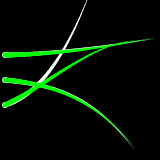
\includegraphics[width=0.075\textwidth]{tracking/frame20.png}
    & 
\includegraphics[width=0.075\textwidth]{tracking/frame30.png}
    \\
    Frame 10 & Frame 20 & Frame 30\\
    
\includegraphics[width=0.075\textwidth]{tracking/frame40.png}
    & 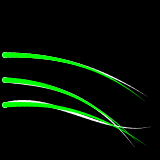
\includegraphics[width=0.075\textwidth]{tracking/frame50.png}
    & 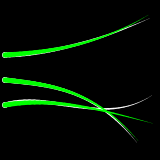
\includegraphics[width=0.075\textwidth]{tracking/frame60.png}
    \\
    Frame 40 & Frame 50 & Frame 60
  \end{tabular}
  \label{tab:result1}

  Table 1: Tracking result using 32 particles on 64 frames of generated whiskers.\\
  White is the whisker being tracked, green is the estimate of its position.
  
\end{center}
